\chapter{Introduction}
\label{ch:intro}

Social insect societies are formed by thousands of individuals, which continuously move and interact with each other inside a dark nest. Honey bee colonies are thus organized complex and dynamical systems, which form a collective intelligence. Observing individual honey bees is, therefore, vital for understanding collective behavior, decision making, and organization of tasks within the colony.

Within the BeesBook\footnote{\url{http://beesbook.mi.fu-berlin.de/wordpress/}; Last accessed: 16.03.2016, 12:05~p.m.} project of the Biorobotics Lab of Freie Universität Berlin~\textcite{wario2015automatic} developed technologies to automatically track all individuals of a honey bee (Apis mellifera) colony. Shortly after birth, each bee has been marked on their thorax using circular 12-bit tags (figure~\ref{fig:markers}) and then added to the colony. The comb is observed by four cameras over a period of nine weeks and each picture is evaluated automatically. The resulting data set contains, for each point in time, the exact position of each bee on the honey comb, its decoded id and its age.

In this thesis, temporal worker-worker interaction networks, based on spatial proximity, are derived from the described data set. Each node in the network is a bee and a link between two individuals is created if they share a position close to each other. The temporal networks are aggregated for several points in time.  Social network analysis methods are applied to determine the usefulness and the characteristics of the resulting networks and its communities.

Until now, social network analysis has been applied to only a subset of a honey bee colonies live, simply because the data were not available to this extent and quality so far.

\begin{figure}[htb]
	\centering
	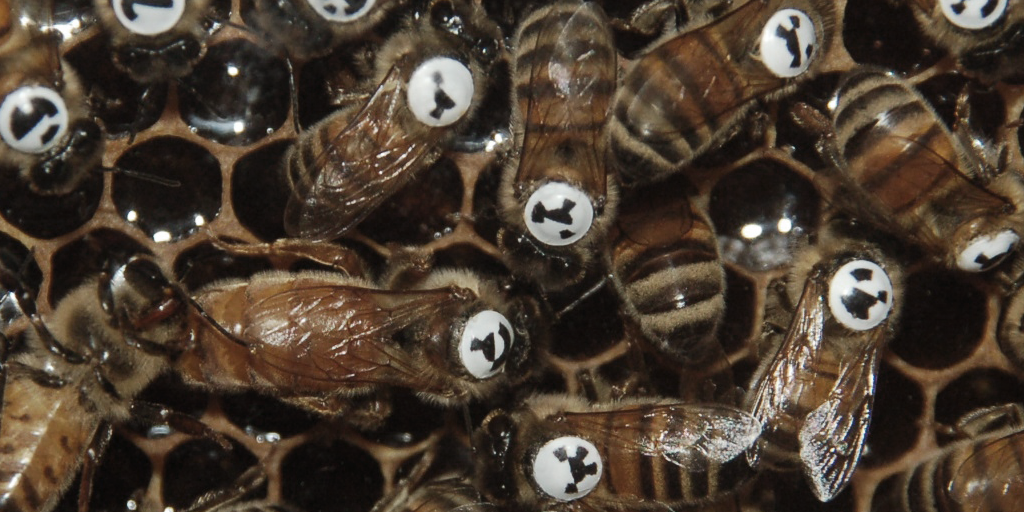
\includegraphics[width=1.0\textwidth]{Figures/markers}
	\caption{Tagged bees inside the hive.}
	\label{fig:markers}
\end{figure}

\section{Motivation}
Most of the studies in the field of animal social network analysis, especially when analyzing the behaviour of social insects colonies, only include a reduced subset of the colonies life, due to a large number of individuals. Usually, the reduction is carried out on three levels (1) time and resolution, (2) space, and (3) number of individuals.

Labeling only a subset of the colonies individuals, a short observation period, low res\-olution and manually extracting information from photos or videos is very common in behavioral sciences~\cite{naug2008structure, quevillon2015social}.

\textcite{baracchi2014socio} observed 300 bees out of a colony with 4000 individuals over a period of ten hours. One of the two sides of the hive was observed by taking a photo each minute. Coloured numbered discs were used for individually marking bees. The analysis of a weighted and undirected worker-worker interaction network revealed a highly compartmentalized structure inside the honey bee colony. Depending on the age, bees occupy different areas of the comb and correspond to different tasks. Also, the contact is limited within groups. \textcite{blonder2011time} color painted all individuals of ant colonies (size 6-90 for each colony) and filmed the colonies for 30 minutes. Interactions between individuals were manually extracted by watching the videos. Using time-ordered (dynamic) networks they analyzed the temporal and spatial dynamics of information flow.

Recently, automated tracking of insects has become technically feasible~\cite{wario2015automatic, crall2015beetag, fiala2005comparing}.
Using automated high resolution tracking data, which includes all individuals of the complete comb over a long time period allows for more advanced analysis focusing on temporal dynamics.
\textcite{mersch2013tracking} automatically tracked all individuals of six ant colonies over a period of 41 days. Applying the Infomap community detection algorithm to the physical contact networks for each day, revealed three distinct and robust groups. Each group represents a functional behavioral unit, with individuals changing groups as they age.

The majority of social insect interaction networks studies, due to previously technical limitations, aggregate temporal tracking data into a single static network~\cite[Chapter~15]{krause2014animal}.
Automatic tracking allows shifting more towards the temporal and dynamic investigation.


\section{Research Goal}

The aim of this thesis is to investigate whether the provided data set of tracked honey bees is useful for creating worker-worker interaction networks using spatial proximity as a proxy for interactions between bees. Thus, I need to implement a pipeline to infer networks out of the data set. Furthermore I want to find out if the resulting networks are suitable for social network analysis.

I want to achieve my research goals by answering the following questions:

\begin{enumerate}
\item \emph{Is it possible to infer networks with the provided honey bee tracking data?}\\
What challenges and limitations does the data set imply? What pipeline parameters are necessary?
\item \emph{What kind of worker-worker interaction networks emerge and how are they structured?}\\
How are those networks characterized and are they different from a random network?
\item \emph{Does the network display a meaningful community structure?}\\
Are those communities robust in terms of pipeline parameters?
\item \emph{How are communities characterized?}\\
Do they reflect known colony behavior in terms of age and spatial distribution?
\item \emph{How do the communities emerge over time?}\\
Are they stable regarding their properties? How do members move between communities?
\end{enumerate}

This work is meant to be the foundation for further more hypothesis-driven research using a network science approach to study the complex system of honey bee colonies and their collective behavior.

\section{Methodology}
The methodology of this thesis follows in the first part a classical explorative data analysis procedure to understand the given data set and estimate its quality. The elaborated characteristics of the dataset are then used to define parameters and steps for the network extraction pipeline. The pipeline is tested, reviewed and refined in an iterative process. The resulting networks are evaluated after each refinement step of the pipeline using the following approaches: (1)~check network properties by investigating the effects of pipeline parameters and features (2)~check network quality using the provided age information of bees, (3)~comparing to a random graph model~(Erdös-Renyi), and (4)~repeatability of known results concerning community structures.

\section{Outline}
This thesis is organized as follows.
Chapter~\ref{ch:bg}, gives a short introduction into social network analysis (SNA) and defines network measures, terms, and algorithms used throughout this work.
In chapter~\ref{ch:relatedwork} a brief summary about the current state of research concerning social insect networks, temporal (dynamic) networks and community detection in animal social networks is given. 
How the networks are derived from the given dataset is described in chapter~\ref{ch:approach}.
Also, the implementation of the network pipeline and its parameters are presented, as well as steps and decisions during the network analyses and community detection process.
The results of the network analysis and the characteristics of the extracted communities are presented in chapter~\ref{ch:results}.
Finally, in chapter~\ref{ch:conclusion} I explore the results and discuss limitations.
I conclude with directions for future work.